



\documentclass[]{report}
\voffset=-1.5cm
\oddsidemargin=0.0cm
\textwidth = 480pt


\usepackage{amsmath}
\usepackage{graphicx}
\usepackage{amssymb}
\usepackage{framed}
\usepackage{multicol}
%\usepackage[paperwidth=21cm, paperheight=29.8cm]{geometry}
%\usepackage[angle=0,scale=1,color=black,hshift=-0.4cm,vshift=15cm]{background}
%\usepackage{multirow}
\usepackage{enumerate}

\usepackage{amsmath,amsfonts,amssymb}
\usepackage{color}
\usepackage{multirow}
\usepackage{eurosym}
\usepackage{framed}

%\input def.tex
%\input dsdef.tex
%\input rgb.tex

%\newcommand \la{\lambda}
%\newcommand \al{a}
%\newcommand \be{b}
\newcommand \x{\overline{x}}
\newcommand \y{\overline{y}}

\begin{document}
	
	\section{3.7 Evolutionary Game Theory}
	The Hawk-Dove game is used in biology to explain why aggression
	is present within populations, but is not always observed.
	Consider the symmetric Hawk-Dove game. The intuition is that
	two indistinguishable individuals must decide whether to share a
	resource or demand the resource for themselves.
	If only one individual demands the resource, then he/she obtains
	that resource (of value v).
	If both demand the resource, they fight. Each wins with probability
	0.5 (thus obtaining the resource). The loser pays a cost of c (due
	to injuries incurred). It is assumed that c > v.
	1 / 46
	
	%======================================================================%
	General Form of the Symmetric Hawk-Dove Game
	The general form of the symmetric Hawk-Dove game is
	H D
	H (0.5[v − c], 0.5[v − c]) (v, 0)
	D (0, v) 0.5(v, v)
	2 / 46
	Evolutionarily Stable Strategies in Symmetric 2-Player
	Matrix Games (ESSs)
	In a symmetric 2-player game, we may define the payoff to a player
	using strategy π1 against a player using strategy π2 to be
	R(π1, π2).
	It is assumed that each player plays a sequence of games, with each
	opponent being chosen at random from the population as a whole.
	Each individual reproduces at a rate proportional to the average
	reward gained in these games (or proportional to some increasing
	function of this average reward).
	It is assumed that the population size is very large (essentially
	infinite).
	3 / 46
	
	%======================================================================%
	Evolutionarily Stable Strategies in Symmetric 2-Player
	Matrix Games (ESSs)
	An ESS, π
	∗ of a symmetric game is a strategy that will be selected
	for when adopted by virtually the whole population. In
	mathematical terms, π
	∗
	is an ESS if
	Either 1) R(π
	∗
	, π∗
	) > R(π, π∗
	), ∀π 6= π
	∗
	or 2) R(π
	∗
	, π∗
	) ≥ R(π, π∗
	), ∀π and if R(π, π∗
	) = R(π
	∗
	, π∗
	) for
	some π 6= π
	∗
	, then R(π, π) < R(π
	∗
	, π).
	4 / 46
	\subsection{Weak and Strong ESSs}
	\begin{itemize}
		\item Any ESS which satisfies Condition 1 is called a strong ESS.
\item A strong, symmetric Nash equilibrium of a symmetric game ⇔
		Strong ESS of symmetric game.
\item Any ESS which does not satisfy Condition 1, but satisfies
		Condition 2 is called a weak ESS.
	\end{itemize}
	
%%	5 / 46
	%======================================================================%
	
	%======================================================================%
	\subsection{Evolutionarily Stable Strategies in Symmetric 2-Player
		Matrix Games (ESSs)}
	The first condition states that if a player knows that an opponent
	will play π
	∗
	, then he/she does strictly better by playing π
	∗
	than by
	playing any other strategy.
	i.e. Any individual playing a different strategy from π
	∗ would be
	selected against.
	The second condition states that if there exists an individual
	mutant (individual not using π
	∗
	) who is not selected against, then
	when the frequency of such mutants is close to zero (but positive),
	then such mutants are selected against.
%%	6 / 46
	%======================================================================%
	\subsection{Evolutionarily Stable Strategies in Symmetric 2-Player
		Matrix Games (ESSs)}
	To see this is the case, suppose that Condition 2 is satisfied and a
	proportion $1 − \epsilon$ play π
	∗
	and a proportion $\epsilon$ play π, where $\epsilon$ is small.
	Since each opponent is chosen from the population as a whole, the
	average reward obtained by π
	∗ players is
\[	R(π
	∗
	,(1 − \epsilon)π
	∗ + \epsilon π) = (1 − \epsilon)R(π
	∗
	, π∗
	) + \epsilon R(π
	∗
	, π).\]
	The average reward obtained by π
	∗ players is
\[	R(\pi,(1−\epsilon)pi
	∗+\epsilon \pi) = (1−\epsilon)R(π, π∗
	)+\epsilon R(π, π) < R(π
	∗
	,(1−\epsilon)\pi
	∗+\epsilon \pi).\]
	If Condition 1 is satisfied, then there is a value $\epsilon_0 > 0$ such that
	this inequality is satisfied for all $\epsilon < \epsilon_0$.
%%	7 / 46
	
	%======================================================================%
	\subsection{Evolutionarily Stable Strategies in Symmetric 2-Player
		Matrix Games (ESSs)}
\begin{itemize}
	\item 	Due to the linearity of the payoff function when a player faces an
	opponent using a mixed strategy, when checking the stability
	conditions we may assume that any mutant uses a pure strategy.
	\item 	It should be noted that at an ESS of a symmetric game, each
	individual should use the same strategy.
	i.e. an ESS of a symmetric game is given by a single strategy,
	while a Nash equilibrium is given by a pair of strategies.
	\item 	Hence, the non-symmetric Nash equilibria [(H, D) and (D, H)] of
	the Hawk-Dove game do not correspond to an evolutionarily stable
	strategy of the Hawk-Dove game.
\end{itemize}

%%	8 / 46
	
	%======================================================================%
\subsection{Relation Between ESSs and Nash Equilibria in Symmetric
	Games}
	An ESS of a symmetric game must correspond to a symmetric
	Nash equilibrium of that game (an ESS of a symmetric game is a
	Nash equilibrium in which both players play the same strategy).
	Hence, the concept of an ESS is a refinement of the concept of a
	Nash equilibrium.
	Any non-trivial 2×2 symmetric matrix game has an ESS.
	Non-trivial - the payoff is essentially dependent on the pair of
	actions taken.
%%	9 / 46
	%======================================================================%
	\subsection{ESSs of Symmetric Matrix Games}
	To derive the ESSs of a symmetric matrix game, we
	1. Find all the symmetric pure Nash equilibria (i.e. Nash
	equilibria where both players always use the same
	action). These are always ESSs (called pure ESSs).
	2. Find the mixed equilibria and check whether they
	satisfy the equilibrium condition (such ESSs are
	called mixed ESSs).
%%	10 / 46
	
	%======================================================================%
	\subsection{ESSs of the Hawk-Dove Game}
	First we look for a pure ESS of the game.
	(H, H) is not a pure ESS, since both players obtain a negative
	expected payoff and by changing unilaterally to D, either one can
	increase their payoff to 0.
	(D, D) is not a pure ESS, since both players obtain v/2. By
	changing unilaterally to H, a player can gain an expected reward of
	v.
	There is no pure ESS. We thus look for a mixed ESS.
	11 / 46
	%======================================================================%
	%======================================================================%
	\subsection{ESSs of the Hawk-Dove Game}
\begin{itemize}
	\item We first look for a mixed Nash equilibrium using the
	Bishop-Cannings theorem.
\item Note any mixed equilibrium of a symmetric 2×2 game is
	symmetric.
\item Suppose the mixed Nash equilibrium is
	[pH + (1 − p)D, pH + (1 − p)D]. When an opponent plays this
	strategy a player is indifferent between H and D.
\end{itemize}	 Hence,
	R(H, pH + (1 − p)D)=R(D, pH + (1 − p)D)
	0.5p(v − c) + (1 − p)v=0.5(1 − p)v ⇒ p =
	v
	c
	12 / 46
	
	%======================================================================%
	%======================================================================%
%%	\subsection{ESSs of the Hawk-Dove Game}
\begin{itemize}
	\item 	Hence, the probability of playing H (level of aggression) is
	increasing in the value of the resource and decreasing in the costs
	incurred in losing a fight.
\item Note that any mixed ESS is by definition a weak ESS.
\item This is due to the fact that when all the population use a strategy
	corresponding to a mixed Nash equilibrium, an individual using an
	action in the support of this equilibrium (or mixture thereof) will
	obtain the same expected payoff as a member of the general
	population.
\end{itemize}

%%-	13 / 46
	
	%======================================================================%
	%======================================================================%
%	\subsection{ESSs of the Hawk-Dove Game}
\begin{itemize}
	\item We now check that Condition 2 for an ESS is satisfied.
	\item This condition states that the ESS strategy must do better against
	any pure strategy than the pure strategy does against itself.
\end{itemize}
	
	Firstly, we check whether an individual using the ESS does better
	against a hawk than a hawk does against another hawk, i.e.
	R(pH + (1 − p)D, H) > R(H, H). We have
\[	R(pH + (1 − p)D, H) = 0.5p(v − c) > R(H, H) = 0.5(v − c),\]
	since p < 1 and v − c < 0.
%	14 / 46
	%======================================================================%
	%======================================================================%
	\subsection{ESSs of the Hawk-Dove Game}
	Secondly, we check whether an individual using the ESS does
	better against a dove than a dove does against another dove, i.e.
	R(pH + (1 − p)D, D) > R(D, D). We have
\[	R(pH + (1 − p)D, D) = pv + (1 − p)v/2 > R(D, D) = v/2.\]
	Hence, pH + (1 − p)D is an ESS.
	15 / 46
	%======================================================================%
	%======================================================================%
	\subsection{Interpretation of Mixed ESSs}
\begin{itemize}
	\item One may ask the following question: does the existence of a mixed
	ESS in which all individuals play H with probability p and play D
	with probability 1 − p mean that there is an equilibrium in which a
	proportion p of individuals always play H and a proportion 1 − p
	always play D?
	\item 	Such an equilibrium is called a stable polymorphism (different
	individuals use different strategies).
	\item 	In the types of game we consider, the answer to the above
	question is ”Yes”. Hence, we can think of a population following a
	mixed strategy as being equivalent to a population in which the
	proportion of individuals using each pure action is equal to the
	probability of using that action under the mixed strategy.
\end{itemize}
	
%%	16 / 46
	
	%======================================================================%
	\subsection{Coordination and Anti-Coordination Games}
	The Hawk-Dove game is an example of an anti-coordination game.
	An anti-coordination game is a symmetric 2×2 game in which
	there are 2 pure equilibria where the players take differing actions.
	In such games the mixed equilibrium is the unique ESS.
	In co-ordination games there are 2 pure, symmetric Nash equilibria
	(i.e. players take the same action at a Nash equilibrium).
%%	17 / 46
	
	%======================================================================%
	\subsection{ESSs in a Co-ordination Game}
	Suppose two individuals play the following game.
\begin{figure}[h!]
\centering
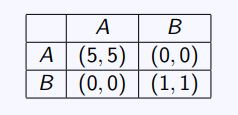
\includegraphics[width=0.5\linewidth]{images/DR7-Slide17}
\caption{}
\label{fig:DR7-Slide17}
\end{figure}

%%	18 / 46
	%======================================================================%
%%	\subsection{ESSs in a Co-ordination Game}
	It is simple to check that (A, A) and (B, B) are strong Nash
	equilibria.
	Hence, both A and B are ESSs.
	There is a mixed Nash equilibrium [pA + (1 − p)B, pA + (1 − p)B],
	where
	R(A, pA + (1 − p)B)=R(B, pA + (1 − p)B)
	5p = (1 − p) ⇒ p =
	1
	6
	.
	
	% 19 / 46
	%======================================================================%
	\subsection{ESSs in a Co-ordination Game}
	We now check whether 1
	6
	A +
	5
	6
	B satisfies Condition 2 for an ESS.
	We first check whether this mixed strategy does better against A
	than A does against itself. We have
	R(
	1
	6
	A + (1 − p)B, A) = 5
	6
	< R(A, A) = 5.
	Hence, 1
	6
	A +
	5
	6
	B is not an ESS. A group of mutants playing A
	would obtain a higher expected payoff (i.e. invade such a
	population).
%%	20 / 46
	%======================================================================%
	\subsection{Replicator Dynamics}
	When there are multiple ESSs, it is natural to ask which one would
	be favoured by natural selection.
	It is clear that this depends on the initial population. If in the
	co-ordination game most of the population are playing A, then the
	population would evolve so that eventually all the population plays
	A.
	Similarly, if nearly all of the population are playing B, then the
	population would evolve so that eventually all the population plays
	B.
	Replicator dynamics are used to simulate the evolution of such a
	population.
%%	21 / 46
	
	%======================================================================%
	\subsection{3.8 Replicator Dynamics in Symmetric Games}
	Suppose players choose one of m actions. The payoff of a player
	when he/she plays Ai and the opponent plays Aj
	is R(Ai
	, Aj),
	where R(Ai
	, Aj) ≥ 0.
	It is assumed that individuals use pure strategies, i.e. they always
	use the same action.
	Let pi,n be the proportion of individuals using action i in
	generation n.
%%	22 / 46
	%======================================================================%
	\subsection{Replicator Dynamics in Symmetric Games}
	Denote the average reward of an individual using action i in
	generation n by Ri,n. We have
\[	Ri,n = R(Ai
	, p1,nA1 + p2,nA2 + . . . + pm,nAm).\]
	Denote the average reward in the population as a whole in
	generation n as Rn. We have
	Rn =
	Xm
	i=1
	pi,nRi,n.
%%	23 / 46
	%==============================================================%
\subsection{Replicator Dynamics in Symmetric Games}
	Individuals using action i are assumed to reproduce in proportion
	to the average reward of these individuals. It follows that the
	proportion of individuals using action i in generation i + 1 is given
	by
	pi,n+1 =
	pi,nRi,n
	Rn
	Varying i from 1 to m − 1, we obtain the replicator dynamic
	equations.
	Note that pm,n = 1 −
	Pm−1
	i=1 pi,n.
	24 / 46
	%==============================================================%
	\subsection{Fixed Points of the Replicator Dynamic Equations}
	A fixed point (p1, p2, . . . , pm) of the replicator dynamic equations
	satisfies
	pi =
	piRi
	R
	, ∀i = 1, 2, . . . , m.
	where Ri and R denote the average reward of individuals taking
	action i and of the population, respectively.
	25 / 46
	%======================================================================%
	\subsection{Fixed Points of the Replicator Dynamic Equations}
	\begin{itemize}
		\item 	It should be noted that all actions that occur with positive
		probability have to obtain the same reward at a fixed point.
		pi = 1, for some i such that 1 ≤ i ≤ m and pj = 0, ∀j 6= i always
		defines a fixed point of the replicator dynamic equations.
		\item A fixed point of the replicator dynamics corresponds to an ESS if
		the fixed point is an attractor.
			\item A fixed point of a dynamic process is an attractor if in some
		neighbourhood of the fixed point, evolution of the system leads to
		the process getting ever closer to that fixed point.
	\end{itemize}

%%- 	26 / 46
	
\end{document}